\chapter{Spiegel AI Remote}
\textit{Erarbeitet von David Vollmer.} \\ \\
Im folgenden wird die \textbf{Spiegel AI Remote} App - auch \textbf{Remote App} genannt - beschrieben. Es handelt sich dabei um eine mobile Anwendung, dessen Hauptaufgabe die Fernsteuerung des Smart Mirrors ist.

\section{Die Flutter\texttrademark{} SDK}
Für die Entwicklung einer mobilen Applikation gibt es heutzutage viele Tool-Kits, die verwendet werden können.
\begin{figure}[h]
    \centering
    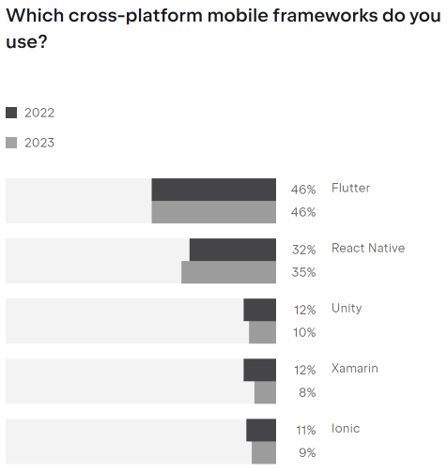
\includegraphics[width=0.4\textwidth]{pictures/frameworks_stats.png}
    \captionsetup{justification=centering, labelformat=simple, singlelinecheck=false}
    \caption{Laut dieser von JetBrains durchgeführten Umfrage war Flutter im Jahr 2023 das am häufigsten verwendete mobile, plattformübergreifende Framework.\cite{jetbrains_survey}}
    \label{fig:jetbrains_survey}
\end{figure} \\
Zusätzlich zu ihrer Popularität ist die von Google entwickelte Flutter SDK in der Lage, mittels AOT-Compiler Programme direkt für die Zielplattform zu kompilieren. Dabei wird die Programmiersprache Dart verwendet.\cite{dart_platform} Flutter unterstützt unter anderem die Entwicklung auf den Plattformen Android SDK, iOS, Windows, macOS und Web.\cite{flutter_supported_platforms} Für die Umsetzung der Fernsteuerungs-App wurde insbesondere mit den Plattformen Android und iOS entwickelt und getestet.

\section{Funktionen}
Um das Display des Spiegel AIs fernzusteuern, müssen einige Hauptfunktionalitäten vorhanden sein. Die Remote App muss in der Lage sein, mit dem Spiegel zu kommunizieren, die Anzeige der Widgets auf dem Display zu ändern, verfügbare Widgets auszuwählen und Profile zu verwalten. Mit Ausnahme der ersten Anforderung, welche in der \textbf{Implementierung} und im Kapitel \textbf{Schnittstelle} näher beschrieben wird, werden all diese Punkte in sogenannten Ansichten (englisch: views) behandelt. Diese kann der Nutzer mithilfe einer Navigationsleiste auswählen.
\begin{figure}[h]
    \centering
    \begin{minipage}[b]{0.27\textwidth}
        \centering
        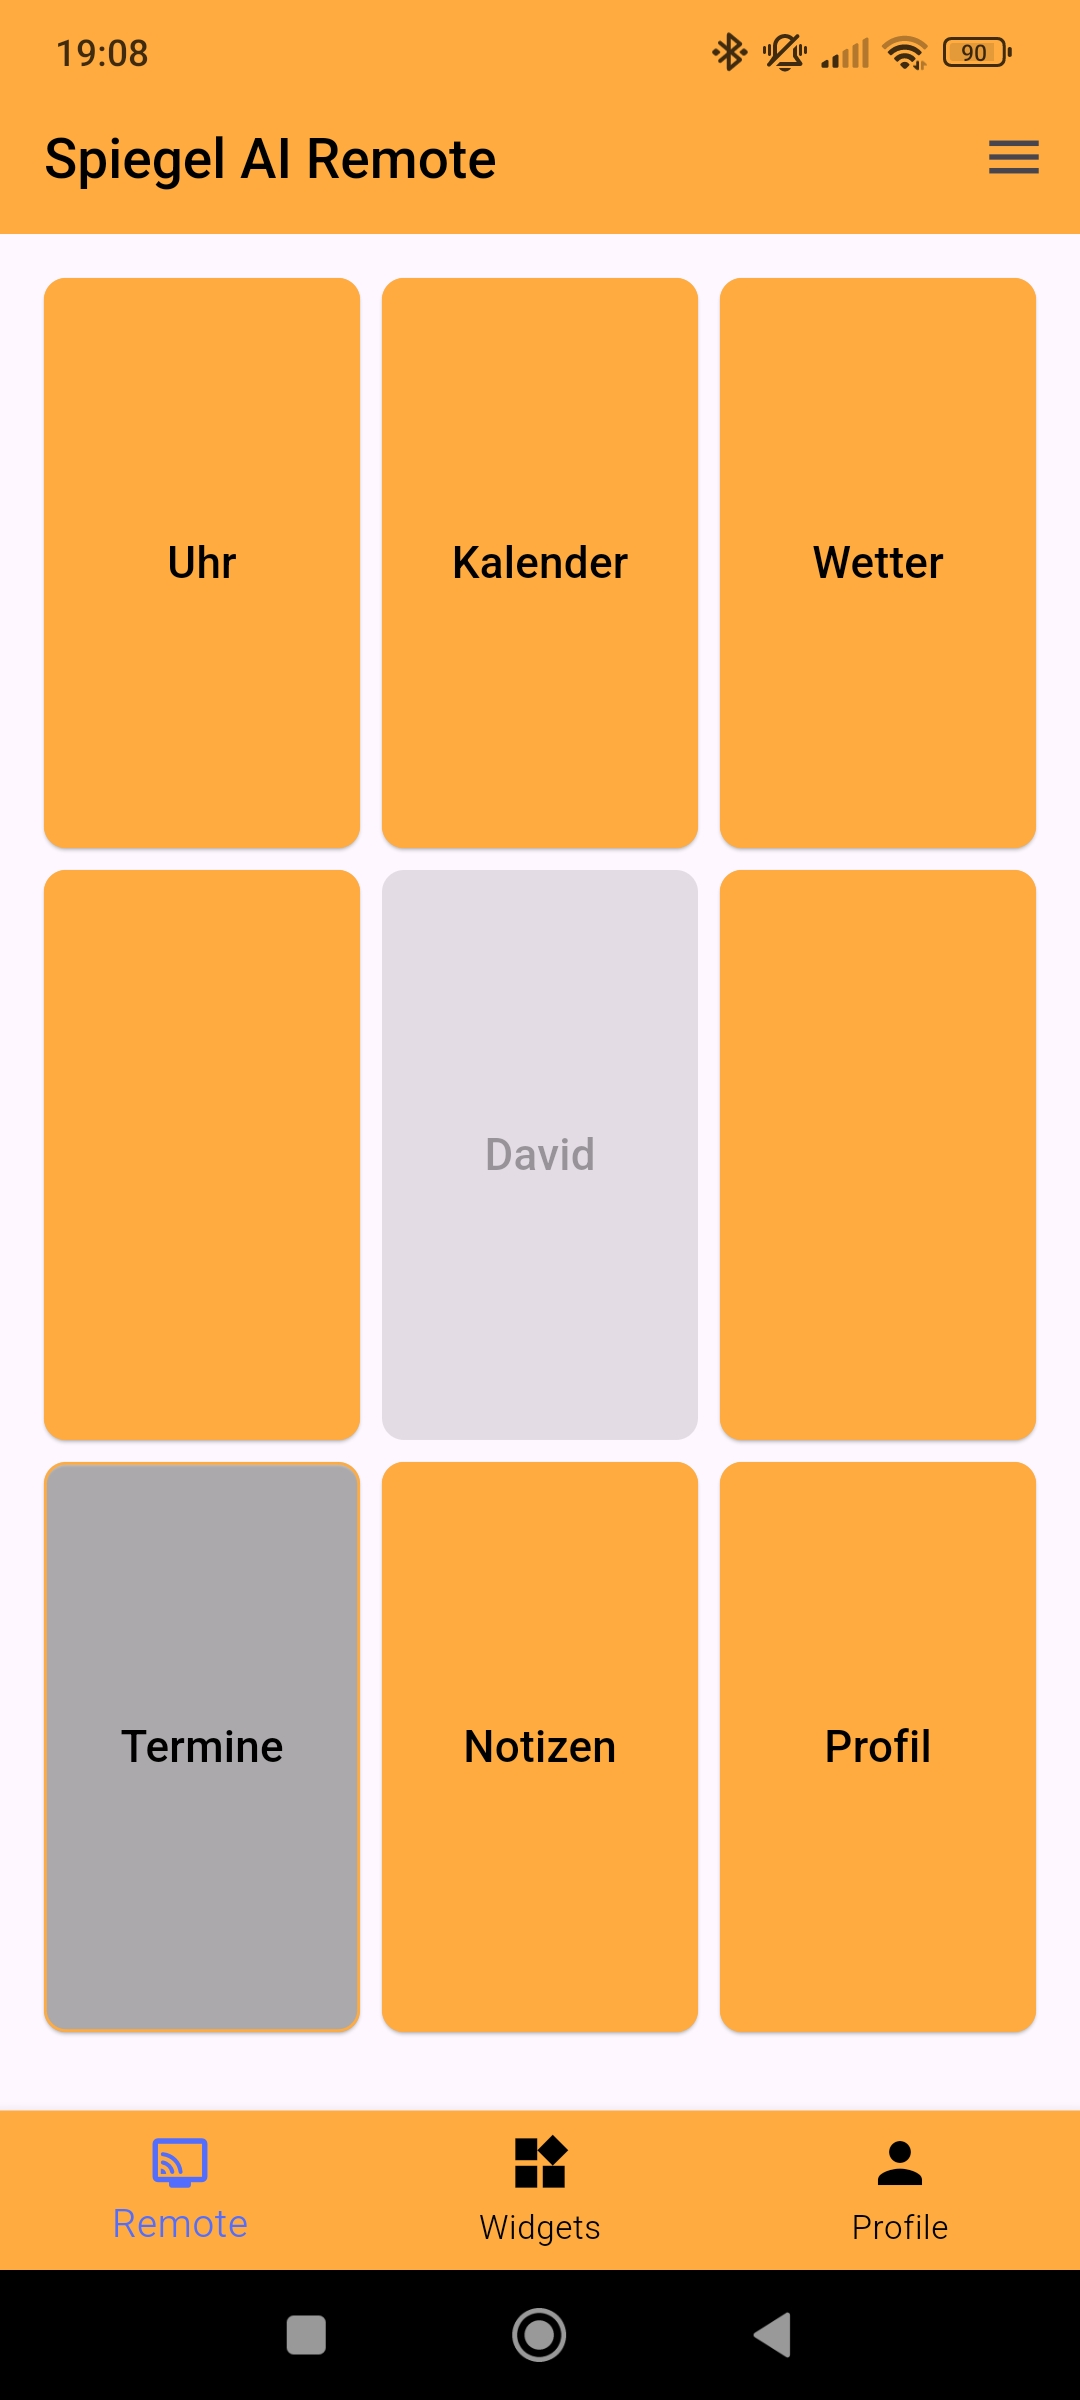
\includegraphics[width=\textwidth]{pictures/remote_remote.jpg}
        \captionsetup{justification=centering, labelformat=simple, singlelinecheck=false}
        \caption{Remote Ansicht}
    \end{minipage}
    \hfill
    \begin{minipage}[b]{0.27\textwidth}
        \centering
        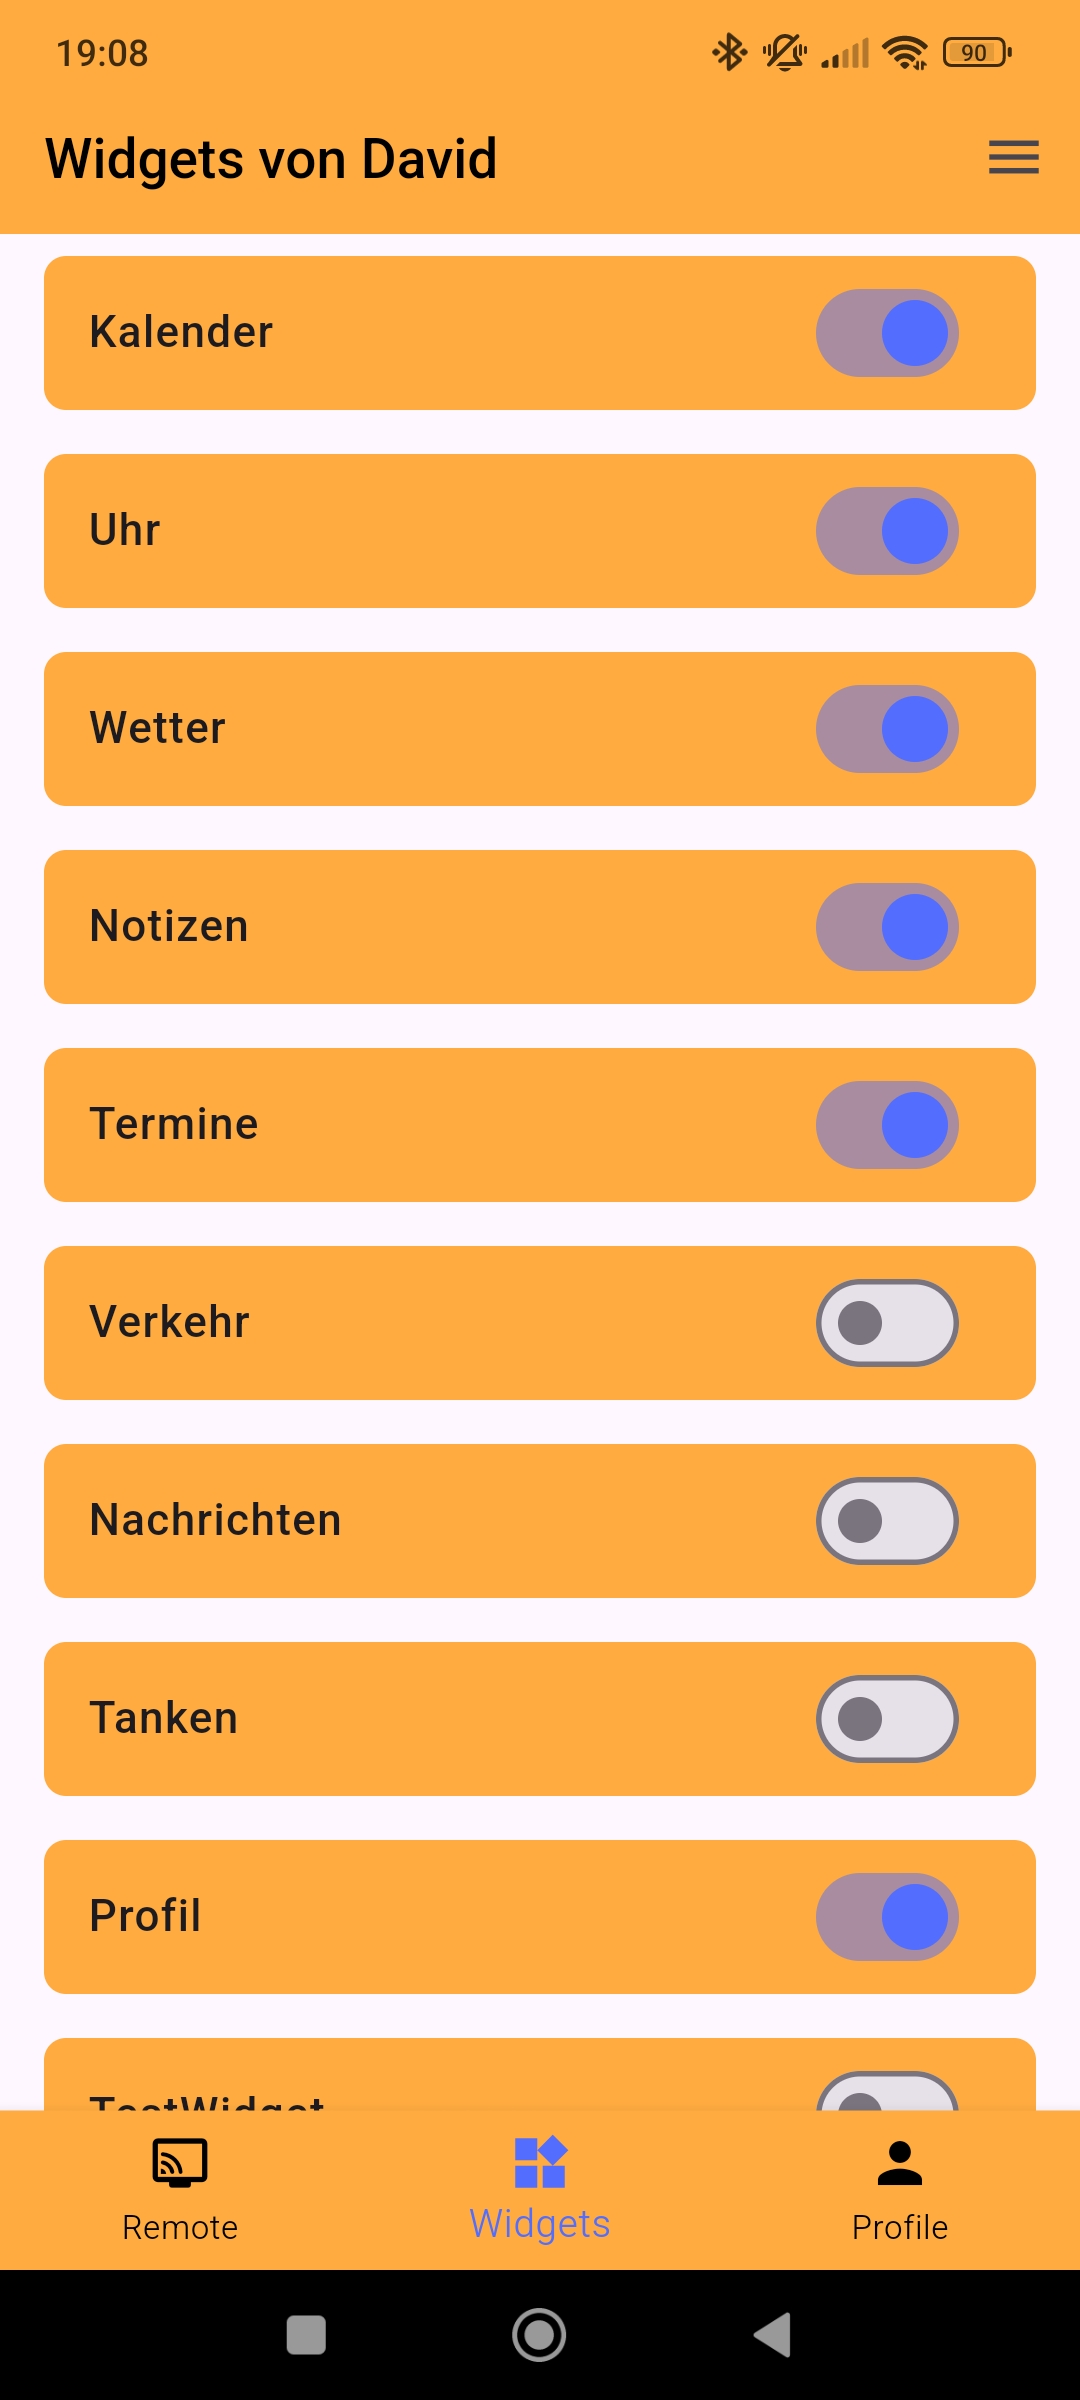
\includegraphics[width=\textwidth]{pictures/remote_widgets.jpg}
        \captionsetup{justification=centering, labelformat=simple, singlelinecheck=false}
        \caption{Widgets Ansicht}
    \end{minipage}
    \hfill
    \begin{minipage}[b]{0.27\textwidth}
        \centering
        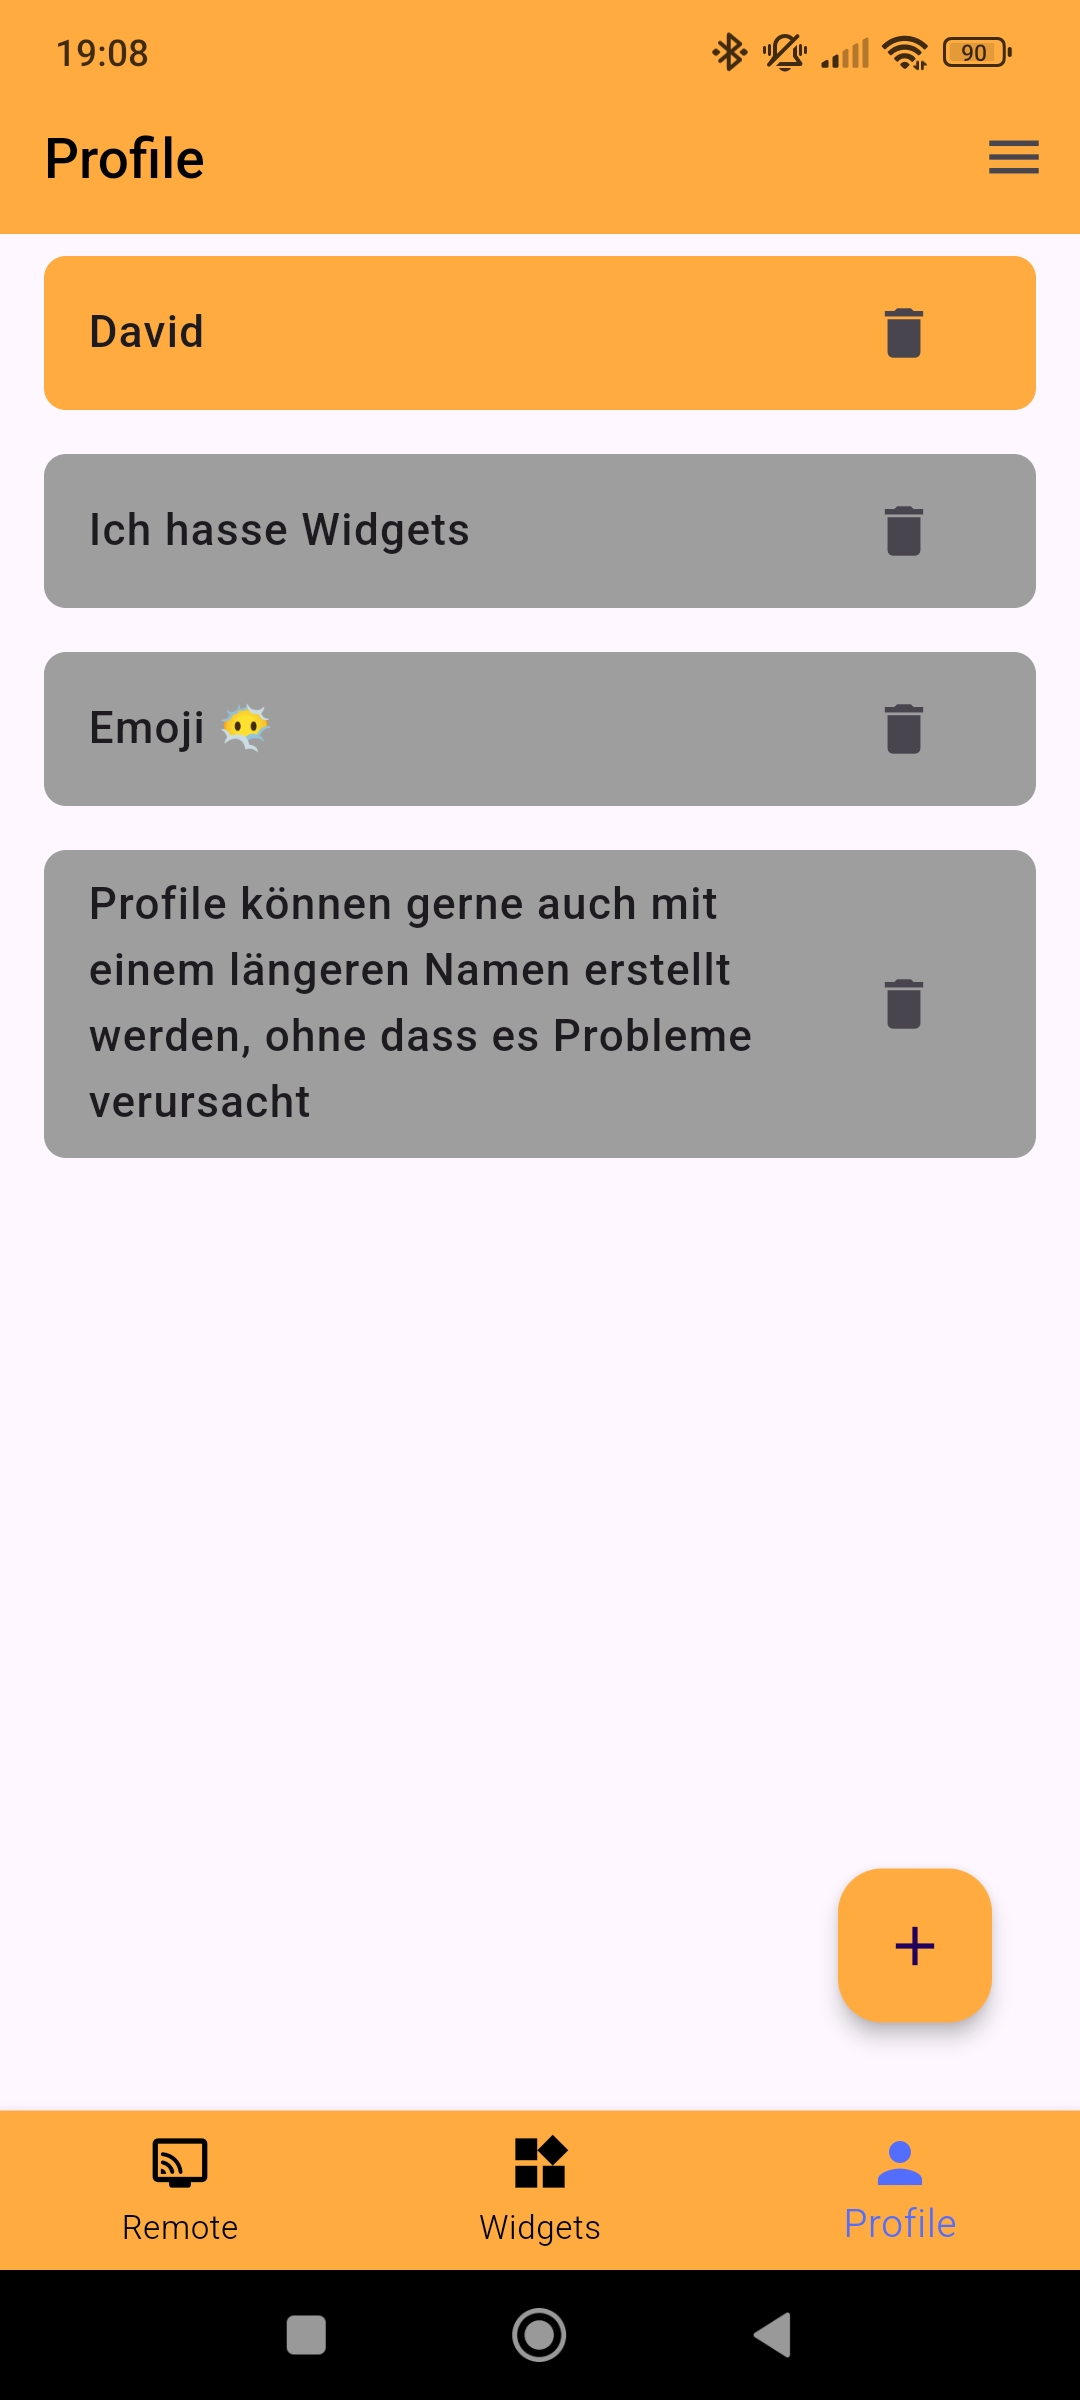
\includegraphics[width=\textwidth]{pictures/remote_profile.jpg}
        \captionsetup{justification=centering, labelformat=simple, singlelinecheck=false}
        \caption{Profile Ansicht}
    \end{minipage}
\end{figure}

\subsection{Remote View}
Die Remote View, welche die Standardansicht nach Öffnen der App ist, bietet die Möglichkeit, den Status der Displayanzeige am Spiegel zu ändern. In der Mitte wird der Name des gerade ausgewählten Profils angezeigt. Dieses Feld lässt keinerlei Interaktion zu, da das zentrale Feld der Spiegelanzeige frei bleibt. Das bedeutet, dass bis zu acht Widgets angezeigt und geändert werden können. Mit einem Klick auf einen Button wird das jeweilige Widget aus- oder eingeblendet. Ein Feld in grauer Farbe bedeutet, dass das Widget vom Spiegel AI Display nicht angezeigt wird. Zieht man ein Widget über ein anderes, werden ihre Positionen getauscht. Die Felder, die keinen Text enthalten, haben die selben Interaktionsmöglichkeiten wie die anderen. Sie sind Platzhalter für Widgets, die hinzugefügt werden können. Falls kein Profil ausgewählt ist, wird im Remote View eine Standardeinstellung angezeigt und jegliche Interaktion der Buttons ist ausgestellt. Bei einem Versuch, ohne Profilselektion eine Änderung vorzunehmen, wird eine Snackbar angezeigt, welche darauf verweist, dass ein Profil geladen sein muss.

\subsection{Widgets View}
In der Widgets Ansicht können für das ausgewählte Profil Widgets ausgewählt werden. Diese View bietet die Widgets Kalender, Uhr, Wetter, Notizen, Termine, Verkehr, Nachrichten, Tanken, Profil und TestWidget an. Bei letzterem handelt es sich um einen Platzhalter, welcher zum Testen der Widgetfunktionalitäten verwendet wurde, aber auch zukünftig mit einem neuen Widget ersetzt werden kann. Die Anwendungen der restlichen Widgets sind im Kapitel \textbf{Display} beschrieben. Mithilfe eines Toggle-Buttons werden bis zu acht Widgets selektiert. Beim Versuch, ein neuntes Widget auszuwählen, schlägt dies fehl und eine Snackbar benachrichtigt über die Obergrenze erlaubter Widgets. Auf die Änderung eines Widgets, ohne ein Profil geladen zu haben, folgt ebenfalls eine dementsprechende Fehlermeldung. Wird ansonsten ein Widget ausgeschaltet, dann wird das im Toggle-Button signalisiert und in der Remote View wird der Name des Widgets mit einem leeren Feld ersetzt. Wenn ein ausgeschaltetes Widget ausgewählt wird, aktualisiert sich auch da der Toggle-Schalter und in der Remote Ansicht wird das erste Feld ohne Textinhalt mit dem Namen des Widgets versehen.

\subsection{Profile View}
Die letzte navigierbare Ansicht ist die Profile View. Hier findet die Verwaltung der gespeicherten Profile statt. Die Profile werden aufgelistet und können mit einem Klick ausgewählt werden. Hält man ein Profil für eine kurze Zeit gedrückt, kann man diese in ihrer Position in der Auflistung ändern, indem man sie an die gewünschte Stelle zieht. Löschen kann man einen Eintrag, indem auf das Mülleimer-Icon geklickt wird. Darauf öffnet sich ein sogenanntes Alert-Dialog, welches das Abbrechen oder Bestätigen der Löschung durchführt. Ein neues Profil kann erstellt werden, indem auf ein Button, welches sich in der Ansicht rechts unten befindet und mit einem '+'-Symbol gekennzeichnet ist, gedrückt wird. Es erscheint ebenfalls ein Alert-Dialog, welches mithilfe eines Texteingabefeldes einen Profilnamen geben kann. Dieser Prozess kann auch abgebrochen oder bestätigt werden. Falls bei Bestätigung der Name des Profils leer oder schon vergeben ist, wird unterhalb des Textfeldes eine entsprechende Fehlermeldung ausgegeben. Wenn das Erstellen des Profils erfolgreich ist, wird das neue Profil direkt ausgewählt und bekommt die ersten acht Widgets in der Widgets View zugeordnet. Sie werden dementsprechend in der Remote Ansicht angezeigt. Alle Anpassungen, die in diesen beiden Ansichten getätigt werden, werden in den jeweilig ausgewählten Profilen gespeichert.

\section{Implementierung}
Der Dart-Code, welcher die Codebase für die Kompilierung des Programms darstellt, befindet sich in einem Flutter-Projekt im Verzeichnis mit dem Namen \enquote{lib}. Der Websocket wird in der \textit{websocket\_manager.dart} verwaltet. Die Funktionalitäten der drei Views sind in den Dateien \textit{remote\_content.dart}, \textit{widgets\_content.dart} und \textit{profile\_content.dart} implementiert.
\begin{figure}[h]
    \centering
    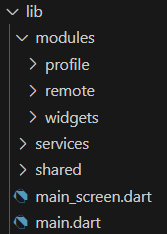
\includegraphics[width=0.2\textwidth]{pictures/flutter_directories.png}
    \captionsetup{justification=centering, labelformat=simple, singlelinecheck=false}
    \caption{Verzeichnisstruktur der \enquote{lib} im Spiegel AI Remote Projekt.}
    \label{fig:flutter_directories}
\end{figure}

\subsection{Websocket}
Um die Kommunikation zwischen der Remote App und Spiegel AI sicherzustellen, muss der Websocket in der App richtig verwaltet werden. Der sogenannte \enquote{WebSocketManager} bewältigt dies mithilfe von Bibliotheken, die die Flutter-Umgebung zur Verfügung stellt. Er ermöglicht, dass eine Verbindung zum Websocket-Server hergestellt und abgebrochen werden kann und erlaubt das Empfangen und Senden von Daten. Die App empfängt Daten als Strings vom Webserver, jedoch werden nur jene mit bestimmten Eigenschaften auch verarbeitet. Der zu empfangende String muss in ein JSON-Format dekodiert werden können. Dann wird geprüft, ob der Wert des ersten Schlüssels mit der Bezeichnung \enquote{sender} den Wert \enquote{mirror} hat. Dies prüft, ob die Nachricht des Servers ursprünglich vom Spiegel AI gesendet wurde. In diesem Fall werden die Werte des Keys mit der Bezeichnung \enquote{profiles} lokal in der App gespeichert. In einem ähnlichen Stil werden Nachrichten versendet. Der einzige Unterschied ist hierbei, dass dabei der \enquote{sender} den Wert \enquote{remote} bekommt, um zu signalisieren, dass die Quelle der Nachricht die mobile Applikation ist. Gesendet werden diese immer, nachdem eine Änderung der Profile stattfindet. Es gibt jedoch eine weitere Nachricht, die die Remote App versendet. Jedes mal, nachdem eine Verbindung mit dem Websocket aufgebaut wurde, sendet sie einen String mit dem Inhalt \enquote{fetch}. Auf die Nachricht folgt, dass der Spiegel AI seinen aktuellen Stand der Profile sendet. Dies ist wichtig, damit die lokalen Profildaten der App synchronisiert werden, bevor sie in der Lage ist, Änderungen vorzunehmen. Ansonsten kann es dazu führen, dass Profildaten des Smart Mirrors mit veralteten Daten der App überschrieben werden. Um sich mit dem Websocket-Server zu verbinden, muss die IP-Adresse und der Port des Servers im Format \enquote{ws://<server-ip>:<server:port>} angegeben werden. Der Websocket schließt, sobald die App entweder geschlossen oder in den Hintergrund laufen gelassen wird. Sobald die App wieder geöffnet wird, wird auch die Verbindung zum Websocket hergestellt und sendet den \enquote{fetch}-String an den Server.

\subsection{Remote}
Die Remote App ist zuständig für die Änderung einer Profileigenschaft mit dem Namen \textbf{state}. Jedes Profil hat einen State, welcher die Positionierung (oder \enquote{index}), ID und Anzeigestatus aller ausgewählten Widgets angibt. Mithilfe dieses Status wird die Anzeige des Spiegels festgelegt. Die Änderungen des States in der Remote Ansicht sind nur am ausgewählten Profil möglich. Ist der Wert der Angegebenen ID \textit{-1}, dann handelt es sich hierbei um ein Feld ohne Widget. Das heißt, es wird an der Stelle kein Name angezeigt und am Spiegel erscheint an dieser Position kein Widget.
\begin{figure}[h]
    \centering
    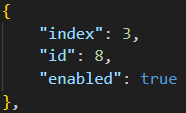
\includegraphics[width=0.35\textwidth]{pictures/remote_state.png}
    \captionsetup{justification=centering, labelformat=simple, singlelinecheck=false}
    \caption{Beispiel eines State-Eintrags im JSON-Format}
    \label{fig:remote_state}
\end{figure} \\
Die Änderung des Anzeigestatus verläuft so, dass nach dem Klick auf einen Button der Wert des Keys \enquote{enable} negiert wird. Ist der Wert \textit{true}, so wird das visualisiert, indem die Farbe des Feldes orange ist. Ist er \textit{false}, dass erscheint es grau. Wird ein Widget über ein anderes gezogen, so werden die Werte ihrer \enquote{index}-Schlüssel getauscht. Dies hat zur Folge, dass sowohl in der Remote Ansicht, als auch im Spiegeldisplay die Positionen geändert werden.

\section{Testen}
Testen